
  En esta sección veremos un caso de estudio usado para verificar la
implementación.
  El problema fue tomado de la competencia SumoUY \cite{sumouy}, el mismo
fue el desafío planteado a escolares en el año 2013.

\section {Problema}

  Se desea implementar un robot autónomo móvil que sea capaz de
hacer la entrega de un pedido en una casa determinada.
  El mismo debe moverse por un escenario e identificar las casas.
  Para recorrer la ruta de entrega, podrá valerse de una línea negra
que representará la calle de la ciudad.

  Las casas estarán ubicadas a un lado de la calle. En el recorrido
se encuentran varias casas, el robot deberá entregar un pedido
en la quinta casa por la que pase.

  El robot deberá pasar por alto las casas anteriores y
al llegar a la casa objetivo debe detenerse totalmente.

  Para probar la solución, se armará un escenario que consiste de
un piso blanco con una línea negra que puede tener curvas.

  Al lado derecho de la línea se ubicarán cajas a menos de 30
centímetros representando las casas.

\section {Solución}

Se armó un robot móvil (Figura \ref{fig:deliverybot}) que cuenta con 3 sensores:

\begin{itemize}
\item Sensor de grises izquierdo
\item Sensor de grises derecho
\item Sensor de distancia apuntando hacia la derecha
\end{itemize}

  Y 2 actuadores:

\begin{itemize}
\item Motor izquierdo
\item Motor derecho 
\end{itemize}

\begin{figure}[hbtp]
\begin{center}
  \caption{Diagrama del robot móvil
    (realizado utilizando fritzing \cite{fritzing})
  }
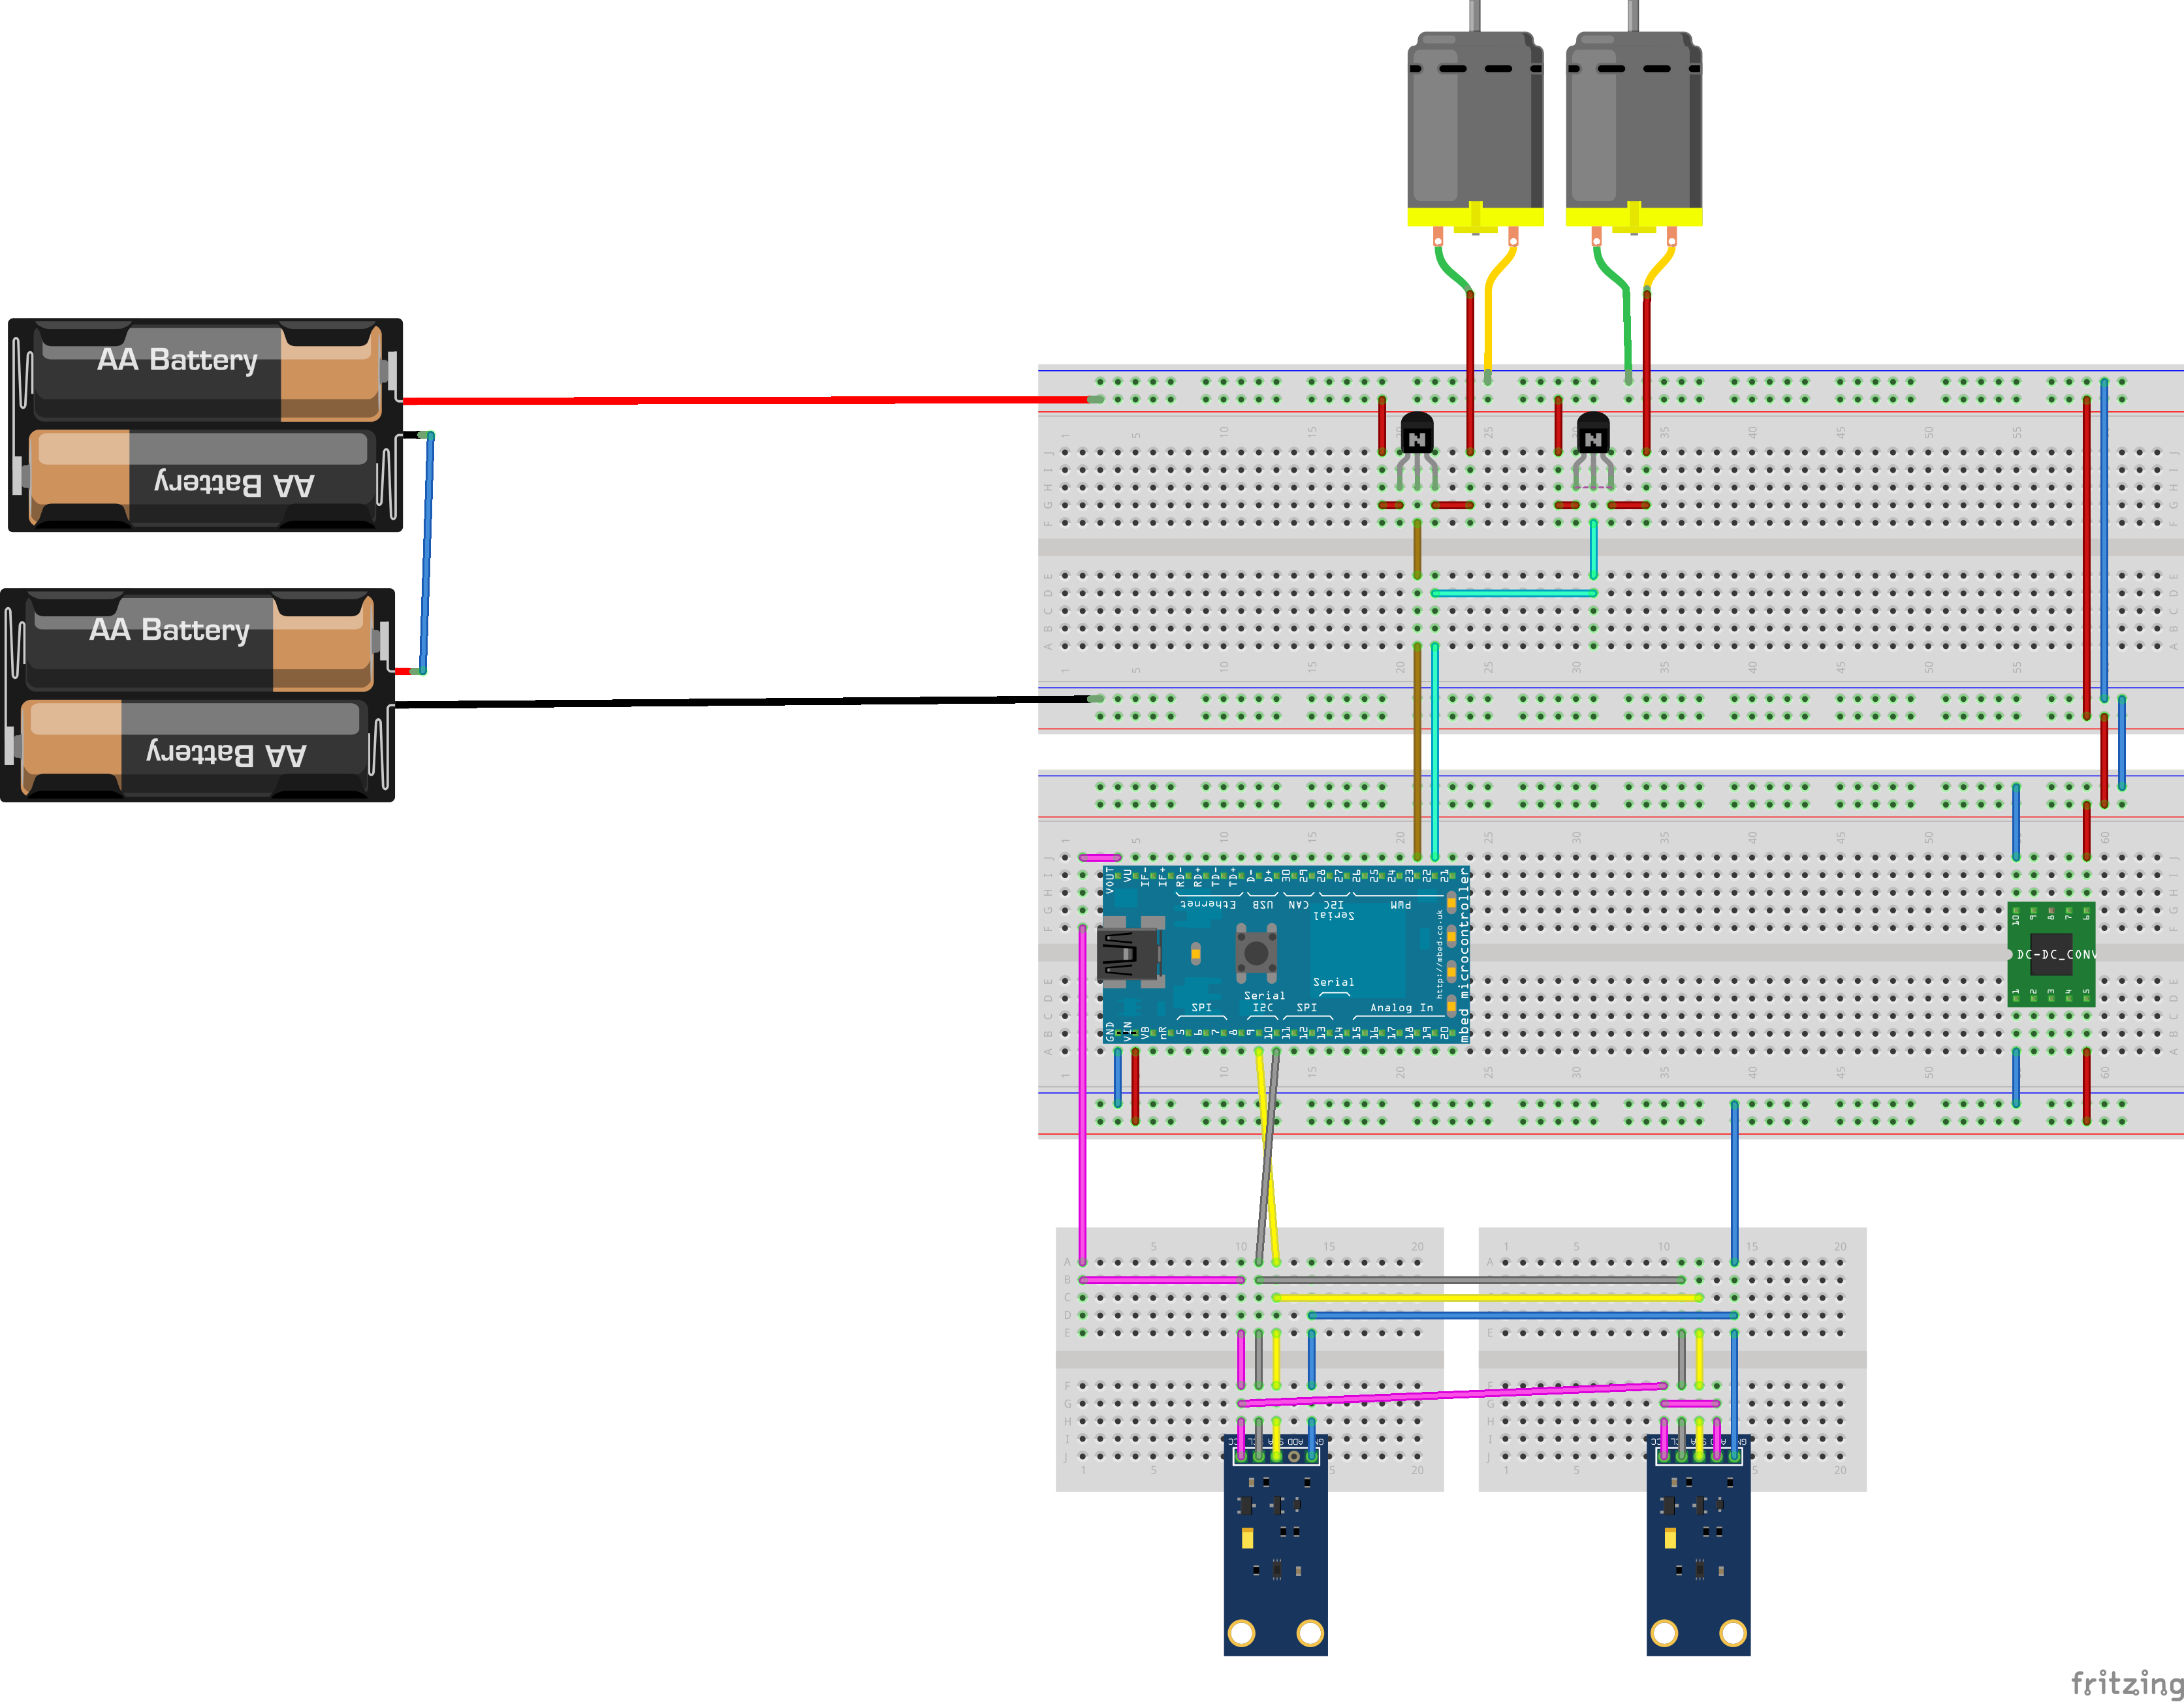
\includegraphics[width=0.9\textwidth]{graphs/breaboardbb.png}
\label{fig:deliverybot}
\end{center}
\end{figure}

  El diagrama muestra los componentes físicos que son montados en el robot
para resolver el problema y cómo se interconectan.
  Arriba se pueden ver los dos motores, que irán uno a cada lado
del robot y sólo se moverán hacia adelante.
  Se utilizan salidas \textit{pwm} \footnote{PWM: Del inglés, pulse width
modulation; Modulación por ancho de pulsos. Se utiliza para crear señales
de voltaje en ciclos periódicos y controlar la cantidad de energía que
se envía.} del MBED para controlar la velocidad de cada motor.

  Los motores necesitan más energía que la que se puede entregar con
los pines de salida del MBED, y para ésto tienen su propia fuente de
voltaje.
  Se utilizan dos transistores para amplificar la señal que
controla cada motor.

  El robot utilizará dos sensores de grises montados al frente
para mantenerse sobre la línea, ambos pueden verse a la derecha abajo
en la figura \ref{fig:deliverybot}.
  Con los motores el robot se moverá hacia adelante inicialmente, e
irá corrigiendo su dirección desacelerando el motor del lado que
se salga de la línea.
  Junto a cada sensor de grises se montará una luz led, que de acuerdo
a el color del suelo, se reflejará y se podrá decidir si se está viendo
algo oscuro (la línea) o algo claro (fuera de la línea).

  El sensor de distancia a la izquierda debajo en la figura, se montará
en el robot apuntando hacia la derecha, para saber cuándo el mismo
está pasando frente a una casa.

  Durante el trayecto se mantendrá la cuenta de las casas, y el robot
se detendrá totalmente cuando la cuenta llegue al valor 5.

  En la Figura \ref{fig:robotfisico} se puede ver el
robot físico creado como prototipo para probar el caso de estudio.

\begin{figure}[hbtp]
\begin{center}
\caption{Robot físico implementado}
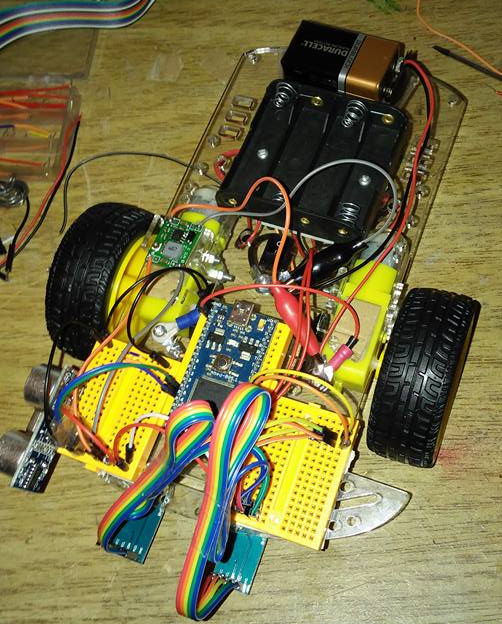
\includegraphics[width=0.9\textwidth]{graphs/alf.jpg}
\label{fig:robotfisico}
\end{center}
\end{figure}


  En la Figura \ref{fig:delivery} se puede ver gráficamente de qué forma
se combinan los eventos para lograr el objetivo.

\begin{figure}[hbtp]
\begin{center}
\caption{Diagrama del caso de estudio}
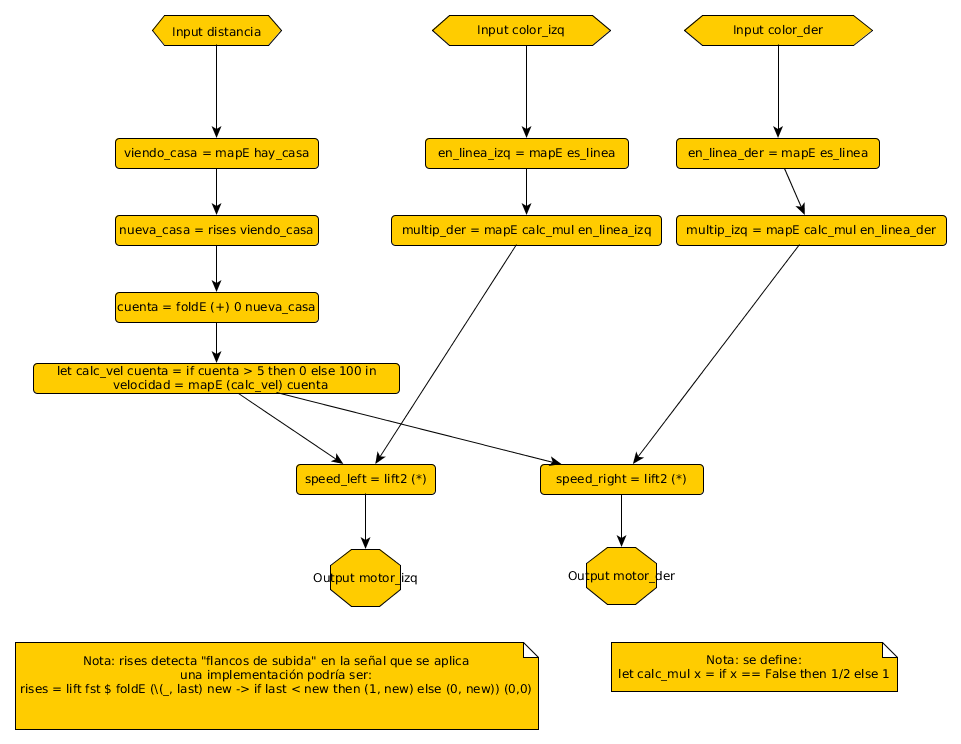
\includegraphics[width=0.9\textwidth]{graphs/delivery.png}
\label{fig:delivery}
\end{center}
\end{figure}

Luego se llega a la implementación en el lenguaje \frob{}:

\begin{verbatim}

INPUT_DISTANCE = 1
INPUT_COLOR_LEFT = 2
INPUT_COLOR_RIGHT = 3
OUTPUT_ENGINE_LEFT = 1
OUTPUT_ENGINE_RIGHT = 2

MIN_DISTANCE = 100
MIN_GREY = 50

hay_casa d = if (d < MIN_DISTANCE) then 1 else 0
distinto a b = if (a /= b) then 1 else 0
velocidad_casa num = if (num >= 5) then 0 else 100

and a b = if (a && b) then 1 else 0
suma a b = (a + b)
multiplicar a b = (a * b)

color_a_vel gris = if (gris > MIN_GREY) 1 else 1/2


do {
    distance <- read INPUT_DISTANCE,
    color_izq <- read INPUT_COLOR_LEFT,
    color_der <- read INPUT_COLOR_RIGHT,

    viendo_casa <- lift hay_casa distance,
    cambio <- folds distinto 0 viendo_casa,
    nueva_casa <- lift2 and viendo_casa cambio,
    cuenta <- folds suma 0 nueva_casa,
    velocidad <- lift velocidad_casa cuenta,

    multip_izq <- lift color_a_vel color_izq,
    multip_der <- lift color_a_vel color_der,

    speed_left <- lift2 multiplicar velocidad multip_izq,
    speed_right <- lift2 multiplicar velocidad multip_der,

    output MOTOR_IZQ speed_left,
    output MOTOR_DER speed_right
}

\end{verbatim}

%\section{Solución sin utilizar \frob}

%\begin{verbatim}

%\end{verbatim}


\section {Conclusiones del caso}

  A diferencia de un programa imperativo tradicional, en el programa
\frob{} dentro del bloque \texttt{do} se puede ver claramente cómo
se procesan las entradas, para generar los valores de las salidas y
razonar sobre los comportamientos.

  Además al estar obligado a escribir funciones puras, el desarrollador
puede abstraerse mejor al pensar que funciones necesita implementar,
y que entradas tomarán. En un programa imperativo, es normal realizar
operaciones de entrada y salida dentro de cualquier función, lo que
dificulta ver cuándo hay efectos secundarios de invocar cada función.

  Finalmente, no es necesario preocuparse por la concurrencia, sinó
por la semántica del programa, la máquina virtual se encargará de
respetar las definiciones del desarrollador.

  Tampoco es necesario preocuparse por las interacciones de entrada
y salida, ya que por decisión de diseño existen abstracciones en
la máquina bien definidas para cada una.

  Si bien \frob{} es muy diferente a los lenguajes de
programación imperativos tradicionales y ésto puede ocasionar una
curva inicial de aprendizaje pronunciada, finalmente puede enseñar al
desarrollador una forma diferente de razonar y pensar la solución
a los problemas de robótica.
